\documentclass[a4paper,12pt]{article}
\usepackage{graphicx}
\usepackage{amsmath}
\begin{document}
\title{Thoughts Related to Learning Programs}
\author{Irvin Hwang}
\maketitle

\section{Structure in Problem Solving}
What is structure?  In problem solving it is often said a particularly elegant solution takes advantage of the ``structure'' of a problem, but what does this mean?  A related question is what is it about problems that allows us to solve them efficiently (i.e. through techniques other than brute-force search)?  We look at the problem of sorting as a case-study.  In the sorting problem we are given a list of objects on which an unknown total order exists, but can be learned by comparing pairs of objects.  The goal is to gain enough information through comparisons to place the objects in an increasing order.  Perhaps the most naive way of solving this problem is to compare all possible pairs of objects and once the relationship is known between each pair of objects placing them in order is trivial.  One would have to make O($n^2$) comparisons, but we know there are more efficient algorithms for this problem.  

In quicksort one takes a ``pivot'' element and divides all the other elements into two groups, a set of elements smaller than the pivot and a set of elements greater than the pivot (we assume all elements are different for simplicity).  Each group is sorted (recursively) and then one concatenates the two lists together to get a completely sorted list.  What is it that makes this more efficient?  The main thing to note is that every element in the small group is smaller than every element in the large group due to transitivity.  This means we can save on the amount of computation we perform by not having to compare elements of the small group with elements in the big group.

In mergesort one splits a set of elements up into indivdual pieces then recursively merges these pieces pairwise into larger and larger ordered lists.   The merge works by always taking the smallest element between the head of the two lists as the next element of the merged list.  Again we can attribute the efficiency of this algorithm to transitivity since the smaller of the two heads will be smaller than all the items in the list with the larger head.  This means we do not have to compare every item to every other item in the lists.

The point here is that one might say these algorithms take advantage of the structure of the problem and that's why they're more efficient than a brute-force method.  And we see structure is really just a property (transitivity) that contrains the possible values of a relation (the total order) and this relation is what we use to solve the problem.  One could argue that most problems involve reasoning about relationships between objects and finding patterns or structure in these relationships is a fundamental aspect of problem solving.

If we examine the situation in terms of cognition we can imagine people experimenting with the problem and comparing items semi-randomly, but beginning to recognize a pattern that when they find $a<b$ and $b<c$ then it is always the case $a<c$.  This pattern or structure can then be represented as a rule or computation that takes two inputs $a<b$ and $b<c$ and produces an output $a<c$.  The question then is how do people recognize this structure or abstract out this rule/computation based on experience?

\section{Patterns and Computation}
  Human survival is dependent on the ability to model and reason about our environment.  If the data we received from our senses was completely random, if the world had no structure or pattern, we would be unable to deal with the complexity of our surroundings given our finite mental resources.  The fact that the world is not random combined with our ability to recognize and reason over patterns is what allows us to exist in this world.  

To get a more concrete sense of what we mean by pattern let us look at
a particular example (Figure \ref{fig:patterns}).  Suppose we have an image like the one below. 
\begin{figure}[htbp]
\begin{center}
%\includegraphics{fig275.pdf}
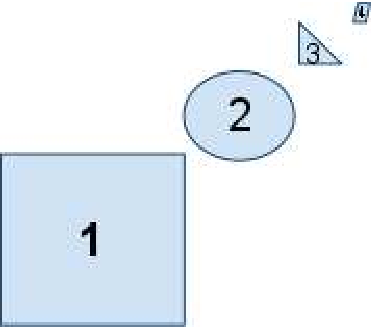
\includegraphics[scale=.5]{patterns.pdf}
\caption{This figure has a pattern of position and a pattern of size. }
\label{fig:patterns}
\end{center}
\end{figure}

This image does not seem randomly generated and most people would
quickly recognize the presence of two patterns 1) the positions of the objects fall on a line and 2) they decrease in
size.  One way to think about these patterns is that they constrain how the data behave.  For example if we were to add an object number five we would probably be able to restrict the possible values for both the position and size of the new object.  What does this mean more formally?  In the case of the first
pattern when we look at the centered position of the objects the
coordinates satisfy a linear relation represented by the computation
$y=mx+b$.  In the second case we see the relation $i<i+1$ holds where $i$ is
the area of the $i$th object.  In both cases we found that a computable
relation held for the data where data in the first pattern were object
positions and data in the second case were areas for the objects.  At
this point one might object to the use of symbols or "rules"
considering these patterns can be recognized without knowledge of the
formal equations.  The important thing to note is the relation that
defines the pattern exists independent of how it is represented and
computed.  Here we represented the relation by computations in a
formal system, but one can also imagine representing the same relation
as computations in a neural circuit etc.  From these examples we can
now intuitively define pattern recognition as finding computations summarizing a relation that constrains the data. 

A computation is essentially any sort of transformation.  There are many formal models of computation such as Turing
machines, the lambda calculus, etc. and there is a widely accepted
hypothesis, the Church-Turing thesis, that any computation (e.g. a computation made by a neural
network) can be expressed in terms of one of these formal models.  Perhaps the best way to think
about computations for our needs is in the language of algorithms and the most common way of representing algorithms is as expressions in some programming
language.  The main difficulty with pattern recognition i.e. finding computations to express relations in data is the space of expressions in a given programming language is huge.  We begin our explorations into pattern recognition by looking at a different, but related problem of how we learn algorithms.

\subsection{Program Induction and Reinforcment Learning}
\subsubsection{Overview}
An algorithm can be thought of as a sequence of actions for solving a problem.  One domain that deals with the process of learning an action sequence for solving a problem is reinforcement learning (RL).  A policy (the output of a reinforcment learning algorithm) can be viewed as a set of computations (action sequences)
that end with the solution to a problem.  An algorithm can be thought
of as a compact representation of the policy that captures the patterns within the set of action sequences.  For example if we revisit the problem of sorting objects one can think of the policy as a map from the known relations between objects and permutations of their order to actions such like comparison and reordering.  Given a particular permutation and no known relationships we can generate an action sequence by taking the action the policy maps to this particular state  and repeating the process with the new state until the goal is reached.   If one were to represent this map as a table it could be quite large depending on the size of the list, but an algorithm for sorting is of constant size and given any list tells the sequence of actions to take in order to reach the goal.

Classical RL algorithms provide a way to learn the mapping from states to actions, but do not scale well due to the exponential growth of the mapping as we increase the complexity of the problem (e.g. by adding features or actions).  These methods roughly work by attempting to estimate the value of an action in a particular state and the policy is defined as taking the actions with the highest value.  While there are methods for dealing with scalability via abstracting over the state space or approximating the value function, the resulting policy seems qualitatively different than what one typically thinks of as an algorithm.

We begin approaching the issue of learning algorithms by tweaking the setup of the problem based on our intuition of algorithms as compact representations of a policy that capture its patterns.  Suppose we already have part of the policy in the form of a set of successful action sequences (sequences of actions that go from an initial state to the goal state).  These might be attained through more traditional reinforcement learning methods and we can imagine this as a sort of dual-process model.  We would like to generalize from these action sequences an algorithm that would produce action sequences with a similar behavior when given a new input.  One possible direction for trying to do this is to look at how an algorithm produces a sequence of actions and then reverse that process.  

An algorithm is typically expressed in a programming language.  The programming language is defined by its syntax and semantics, where the syntax defines what makes an expression in the language and the semantics define how these expressions should be evaluated i.e. what actions to take.  We can roughly think of the semantics as a machine that takes in an expression in the language (an algorithm/program) and and produces a sequence of actions.  The semantics are made up of what are essentially a collection of if-then rules and so if we wish to infer an expression based on actions perhaps we can find the rules where our actions are the consequent (the ``then'' part of the rule) and make our expressions the antecedent (the ``if'' part of the rule).  The problem here is many expressions can evaluate to the same value and so the space of possible expressions would end up being quite large.  One possiblity is to use this approach to generate a sort of naive expression that is essentially a literal translation of the action sequences into an expression and then generalize from this expression into something compact using more sophisticated methods like in the work of Kitzelmann and Schmidd \cite{Kitzelmann2006Inductive}.  Another possible direction for the use of semantics is as a way to define the neighborhood relation in a sampling method such as MCMC where expressions are connected by the traversal through the semantics.

\subsection{Possible Approaches and Technical Issues}
We propose working on a series of succesively complicated problems in order to better understand the issues related to program induction.  To demonstrate the approach we begin with the simple set-up of an RL problem with a single binary reward, a single binary action, a single binary feature, and we assume the Markov assumption holds in the sense the reward at a given time-step is only dependent on the feature of that time-step.  One should be able to express the algorithm for this problem as a single if expression conditioned upon the value of the single feature.

The first issue we must address is what language to choose in order to model the problem.  Ideally one would be able to start from the lambda calculus and then learn useful syntax such as conditional expressions and booleans based on the problems one faces, but to simplify things let us assume we already have a syntax with these constructs.  There are still many questions involved related to the language such as whether the language should be imperative or functional.  On the one hand it seems natural to use semantics for an imperative language like in Winskel's text \cite{Winskel1993Formal} where the semantics for commands would correspond to actions in the RL setting and access and maintainence to state information can be modeled as accessing memory.  On the other hand programming language semantics seem to be more developed for functional languages \cite{Pierce2002Types} and inference on functional semantics seems like it may be cleaner due to referential transparency.  This question brings up more abstract issues such as whether cognition should be modeled as stateful computation since we have memory or whether a functional approach is better since it seems easier to map functional computation (everything determined by input and output to computational units) to a neural circuit-like conception of cognition.  More concrete issues involve how input and actions from the world should be modeled in the language.  Should we include variables through a let construct in the language and let specific actions and inputs be values an action/input variable can take?  Or should we keep things simple and just have specific actions and inputs as syntactic primitives much like True or False and try to work with them that way.  There are also many questions of how search should proceed. 

To demonstrate some of the issues related to search, suppose we start with the following language:
\begin{align*}
exp ::= &\texttt{ True} \\
    |& \texttt{ False} \\
    |& \texttt{ If } exp \texttt{ }exp \texttt{ } exp \\
    |& \texttt{ Unknown }\\
    |& \texttt{ Act }\\
    |& \texttt{ NoAct }\\
    |& \texttt{ On }\\
    |& \texttt{ Off }\\
    |& \texttt{ Action }\\
    |& \texttt{ Feature }\\
    |& \texttt{ == }exp \texttt{ }exp
\end{align*}

A general idea of how the semantics might be defined is listed below

\begin{eqnarray}
&\frac{}{\texttt{if True } exp_1\texttt{ } exp_2 \rightarrow exp_1}\label{ifTrue}&\\
&\frac{}{\texttt{if False } exp_1\texttt{ } exp_2 \rightarrow exp_2} \label{ifFalse}&\\
&\frac{\text{feature-action pair is } (\_,\text{NoAct})}{== \texttt{ Action } \texttt{Act} \rightarrow \texttt{False}} &\\
&\frac{\text{feature-action pair is } (\text{On},\_)}{== \texttt{ Feature } \texttt{On} \rightarrow \texttt{True}} \label{fOn} &\\
&\frac{}{\texttt{Act} \rightarrow \text{Act}} \label{action}&
\end{eqnarray}

Imagine we have a couple of action sequences (in our particular case each action sequence ((features,action),...,(features,action))  will only be of length one) $\{\text{((On,Act)), ((Off, NoAct))}\}$.  Suppose we infer from ((On,Act)) the expression \texttt{Act} using (\ref{action}) and from this expression we get \texttt{If True Act Unknown} using (\ref{ifTrue}).  We also know that when the action the action Act was taken the input/feature had the value On so \texttt{== Feature On} would evaluate to \texttt{True} by (\ref{fOn}).  Is there a principaled way of guiding the search so that inference from \texttt{If True Act Unknown} goes to \texttt{If (== Feature On) Act Unknown} using (\ref{fOn})?  Let us also suppose for the input-action pair \texttt{(off,no action)} we infer \texttt{If False Unknown NoAct} using (\ref{ifFalse}), can we guide inference to combine our hypotheses \texttt{If (== Feature on) Act Unknown} and \texttt{If False Unknown NoAct} into \texttt{If (Feature==On) Act NoAct}.

A natural next step is to look at problems that require a sequence of actions in order to reach the solution rather than a single action.  Interesting questions that arise are how syntactic constructs such as loops or recursion relate to problems of learning sequences.  One can think of an MDP as having an implicit loop that runs until reward is received and at each step we refer to a policy that is a conditional expression that tells what action to take based on the features of the current state.  In some sense the Markov assumption tells us we don't need to do anything more complicated than have a running for loop where we condition on the features of the current state, but in day-to-day life there seems to be much more variablility in how algorithms are expressed.  Perhaps a more formal understanding of this situation would help develop how to think about infer expressions for more complicated problems.
\bibliographystyle{plain}
\bibliography{myBib}
\end{document}
